\documentclass{article}
\usepackage[utf8]{inputenc}
\usepackage{graphicx}
\usepackage{usecases}

\title{Team- Sole survivors}
\author{kirandeep kaur(740003), Gurjot Singh(735957), Xiao Wu(727686}
\date{}

\usepackage{natbib}
\usepackage{graphicx}

\begin{document}

\maketitle

\section{Statement Of Work}
Creating Use Cases for a sample Racing Game
\subsection{Requirements}
The System shall provide the user:

\begin{enumerate}
    \item  Requirement 1: Registering to the player Database and Validating their Login
    \item  Requirement 2: Giving them a choice for a vehicle
    \item  Requirement 3: Control Over the vehicle to race against System Generated vehicles

\end{enumerate}


\begin{figure}[h!]
\centering
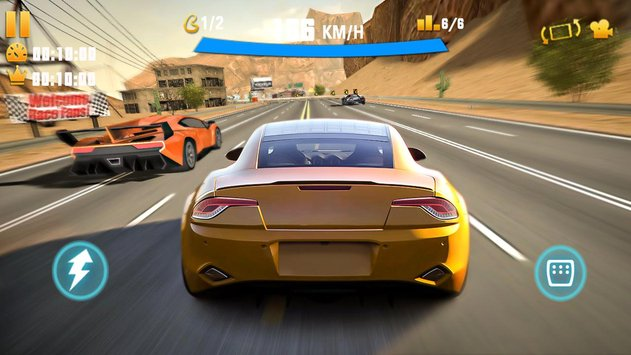
\includegraphics[scale=0.5]{car}
\caption{The Racing Games}
\label{fig:car}
\end{figure}


\pagebreak
\section{Use Cases}
\subsection{Use Case 1: Registering to the player Database}
\subsubsection{PreCondition: User is not registered}
\subsubsection{GOAL}
To enable user registeration to the database

\begin{figure}[h!]
\centering
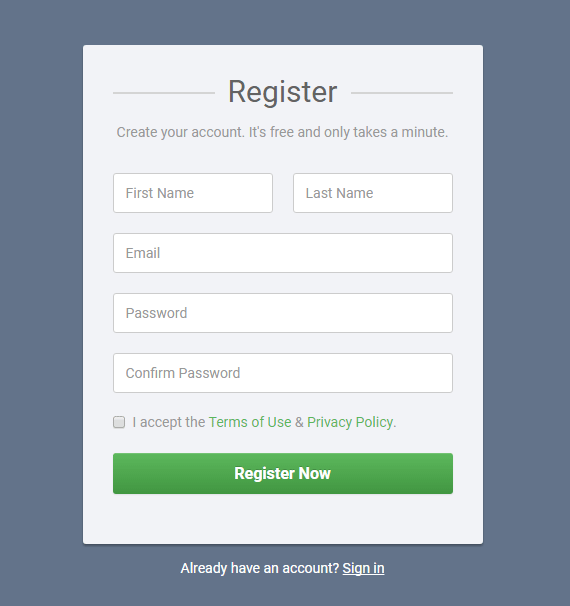
\includegraphics[scale=0.5]{register}
\caption{The Registration process}
\label{fig:register}
\end{figure}

\subsubsection{Actor}

\begin{enumerate}
    \item  User
    \item  Database Management System

\end{enumerate}
\subsubsection{Scenario}

\begin{enumerate}
    \item  Step 1. The System Provides a UI for the User to Enter his Details for Registration to the Application Database
    \item  Step 2. The User enters his details in the required fields such as userName, userId, Contact etc.
    \item  Step 3. The System sends the entered values to the Database to be stored
    \item  Step 4. Database Management system stores the values in required columns

\end{enumerate}

\subsubsection{UML 1:}
\begin{enumerate}
    \item Registration
    \item Data Members (Nouns)
          \begin{enumerate}
              \item userName
              \item userId
              \item contact
          \end{enumerate}
    \item Behaviour
        \begin{enumerate}
            \item Generate Register UI
            \item Create Table in the Database
            \item Pass Values To the table
        \end{enumerate}
\end{enumerate}

\subsection{Use Case 2: Validating User Login}
\subsubsection{PreCondition: User is already registered}
\subsubsection{GOAL}
To enable user SignIn into system with their registered username and password.

\begin{figure}[h!]
\centering
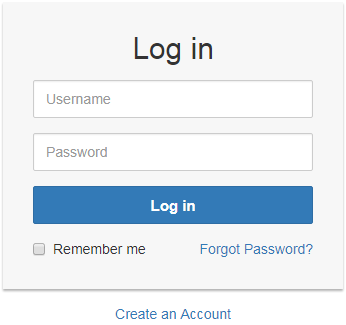
\includegraphics[scale=0.5]{login}
\caption{The login process}
\label{fig:login}
\end{figure}

\subsubsection{Actor}

\begin{enumerate}
    \item  User
    \item  Database Management System

\end{enumerate}
\subsubsection{Scenario}

\begin{enumerate}

    \item  Step 1. System provides a UI to the user to SignIn 
    \item  Step 2. User enters his username/password
    \item  Step 3. System validates entered values against the database
    \item  Step 4. If successful, the user is given access to the game server

\end{enumerate}


\subsubsection{UML 2:}
\begin{enumerate}
    \item Login
    \item Data Members (Nouns)
          \begin{enumerate}
              \item userName
              \item Password
              
          \end{enumerate}
    \item Behaviour
        \begin{enumerate}
            \item Provide Login UI
            \item Validate user entered Values against Database Table
            \item Give user access to game server
        \end{enumerate}
\end{enumerate}

\subsection{Use Case 3 : Giving them a choice for a vehicle}
\subsubsection{PreCondition: User has already Logged In}

\subsubsection{GOAL}
To provide different options to user to choose a vehicle from database

\subsubsection{Actor}

\begin{enumerate}
    \item  User
    \item  Database Management System

\end{enumerate}
\subsubsection{Scenario}

\begin{enumerate}

    \item  Step 1. The System provides a UI with a list of vehicles with images from databases
    \item  Step 2. The User makes a choice and submits it to the system

\end{enumerate}

\subsubsection{UML 3:}
\begin{enumerate}
    \item Options
    \item Data Members (Nouns)
          \begin{enumerate}
              \item ListOfCars
              \item carImageList
              
          \end{enumerate}
    \item Behaviour
        \begin{enumerate}
            \item Get image name from database
            \item Show vehicle list with images to user
            \item Pass selected values to next screen.
        \end{enumerate}
\end{enumerate}

\subsection{Use Case 4: Control Over the vehicle to race against System Generated vehicles}

\subsubsection{GOAL}
to give user access and control over his chosen vehicle that can be used for the game via an input device (such as keyboard).

\begin{figure}[h!]
\centering
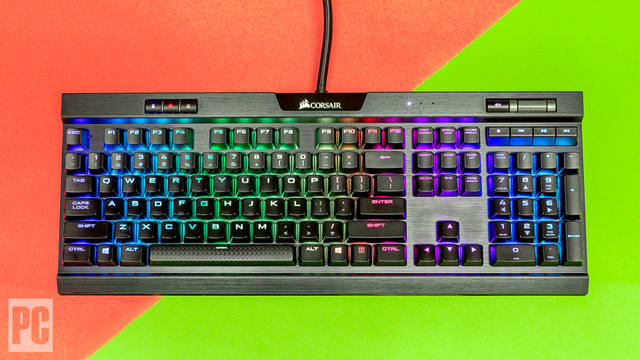
\includegraphics[scale=0.4]{keyboard}
\caption{The Input Device - Keyboard}
\label{fig:keyboard}
\end{figure}

\subsubsection{Actor}

\begin{enumerate}
    \item  User
    \item  Database Management System

\end{enumerate}
\subsubsection{Scenario}

\begin{enumerate}
    \item Step 1. The System allows input from user's input device(keyboard)
    \item Step 2. Depending on the key inputs the vehicle changes direction to allow user full control over it

\end{enumerate}

\subsubsection{UML 4:}
\begin{enumerate}
    \item Control
    \item Data Members (Nouns)
          \begin{enumerate}
              \item userInput
             
          \end{enumerate}
    \item Behaviour
        \begin{enumerate}
            \item get user input
            \item Move vehicle according to user input
        \end{enumerate}
\end{enumerate}

\pagebreak
\bibliographystyle{plain}

\end{document}
